\documentclass[11pt,a4paper]{scrartcl}
\usepackage[T1]{fontenc}
\usepackage{microtype}
\usepackage{lmodern}
\usepackage{amsmath}
\usepackage{amsfonts}
\usepackage{amssymb}
\usepackage{enumerate}
\usepackage{graphicx}
\usepackage{float}

\usepackage{listings}
\usepackage{color}
%% http://stackoverflow.com/questions/741985/latex-source-code-listing-like-in-professional-books
\usepackage{courier}
\definecolor{light-gray}{gray}{0.95}
\lstset{
  % language=C,
  basicstyle=\small\sffamily,
%   basicstyle=\small\ttfamily,
  numbers=left,
  numberstyle=\tiny,
  frame=tb,
%  columns=fullflexible,
%  showstringspaces=false,
	backgroundcolor=\color{light-gray},
	linewidth=\linewidth,       % Zeilenbreite
	breaklines=true,             % Zeileumbruch
	breakatwhitespace=false, %Umbruch an Leerzeichen
  tabsize=2,
  extendedchars=true,
  xleftmargin=17pt,
  framexleftmargin=17pt,
  abovecaptionskip=7pt,
%   frameround=tttt,
}

\def\ojoin{\setbox0=\hbox{$\bowtie$}%
  \rule[-.02ex]{.25em}{.4pt}\llap{\rule[\ht0]{.25em}{.4pt}}}
\def\leftouterjoin{\mathbin{\ojoin\mkern-5.8mu\bowtie}}
\def\rightouterjoin{\mathbin{\bowtie\mkern-5.8mu\ojoin}}
\def\fullouterjoin{\mathbin{\ojoin\mkern-5.8mu\bowtie\mkern-5.8mu\ojoin}}

\begin{document}

\author{Johannes Merkle\\Ralf Vogler}
\title{Query Optimization}
\subtitle{11. Exercise}

\maketitle

\section*{Exercise 1 - Binomial coefficient}
\begin{align}
Definition: \begin{pmatrix} n \\ k \end{pmatrix} = \frac{n!}{k! \cdot (n-k)!}\\
\begin{pmatrix} n \\ n-k \end{pmatrix} = \frac{n!}{(n-k)! \cdot (n-(n-k))!} = \frac{n!}{(n-k)! \cdot k!} = \begin{pmatrix} n \\ k \end{pmatrix}
\end{align}


\section*{Exercise 2 - Accessed pages (manually)}
$m = 3, n = 2, N = nm = 6, k = 2$\\
-> Average number of accessed pages for reading 2 tuples?\\
Possiblities how our k tuples are located (bit vector where 1 is a tuple we want, others are 0. "|" separates pages):\\
\begin{tabular}{|c|c|}
\hline
Tuples & Accessed pages\\
\hline
00|00|11 & 1\\
00|11|00 & 1\\
11|00|00 & 1\\
00|01|01 & 2\\
00|01|10 & 2\\
00|10|01 & 2\\
00|10|10 & 2\\
01|00|01 & 2\\
01|00|10 & 2\\
10|00|01 & 2\\
10|00|10 & 2\\
01|01|00 & 2\\
01|10|00 & 2\\
10|01|00 & 2\\
10|10|00 & 2\\
\hline
\end{tabular}\\
We have 3 * tuples on the same page and (L-3) * tuples on different pages\\
with L = \#possible distributions = $\begin{pmatrix} N \\ k \end{pmatrix} = \begin{pmatrix} 6 \\ 2 \end{pmatrix} = 15$.\\
$Average = (3*1 + 12*2)/15 = 1.8$\\

\section*{Exercise 3 - Yao formula for optimization}
\begin{lstlisting}[language=SQL]
select * from student s where s.age>20
\end{lstlisting}
Assume we have an clustered index on \textit{age}. When using the index we go down the tree and find the first tuple for which the predicate holds, then we go through the leaves to get the other tuples until the predicate is no longer true.
To read each tuple we have to jump around on the disk - moving the head with a certain seek time.

Using Yaos formula we can calculate the expected number of pages we have to access.
Assuming a certain seek time and bandwith for the drive, we can then calculate (like in Ex 10.2) wether it's faster to use the index or to do a tablescan.



\section*{Exercise 4 - Plot: Yao, Bernstein, Waters}
$m = 100, n = 10, N = nm = 1000, k = 1:N$\\
The file \verb|ex4.m| contains Matlab code for generating the following plots.\\
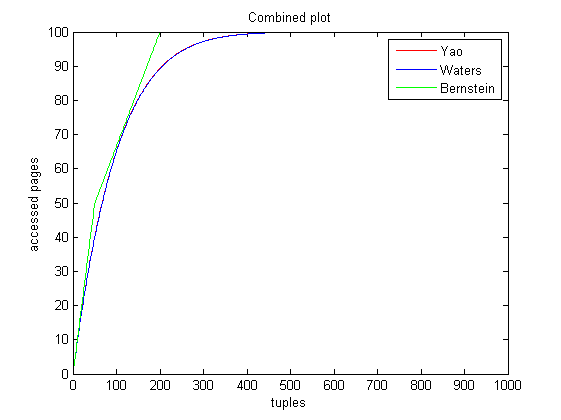
\includegraphics{combined}\\
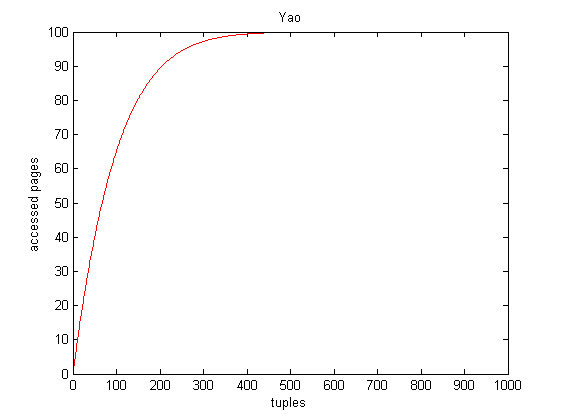
\includegraphics[scale=.9]{yao}\\
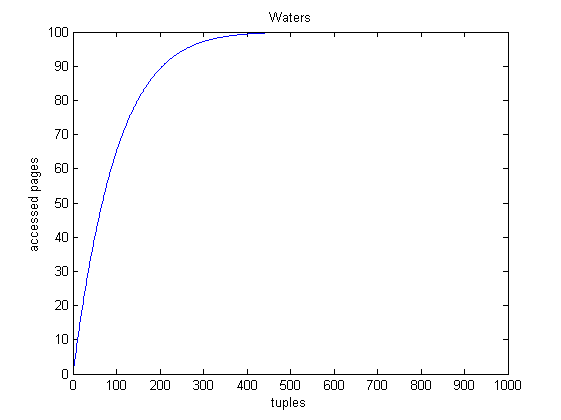
\includegraphics[scale=.9]{waters}\\
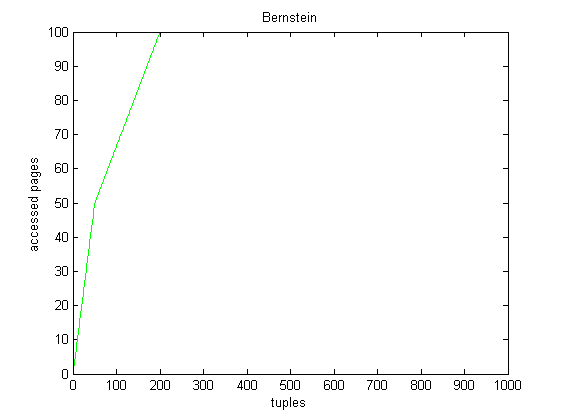
\includegraphics[scale=.9]{bernstein}

\lstinputlisting[language=Matlab,caption={Matlab code},label=lst:ex4]{ex4.m}

\end{document}
